\documentclass{article}
\usepackage{xcolor}
\usepackage{tikz}
\usepackage{graphicx}
\usepackage[hidelinks]{hyperref}
\usepackage{listings}
\usepackage{float}
\usepackage{pdfpages}
\usepackage{tcolorbox}
\usepackage{textcomp}

\definecolor{light-gray}{gray}{0.9}
\lstset{frame=tb,
extendedchars = true,
texcl=true,
  language=bash,
  aboveskip=3mm,
  belowskip=3mm,
  frame=none,
  backgroundcolor=\color{light-gray},
  showstringspaces=false,
  columns=flexible,
  basicstyle={\small\ttfamily},
  numbers=none,
  numberstyle=\tiny\color{gray},
  keywordstyle=\color{blue},
  stringstyle=\color{mauve},
  breaklines=true,
  tabsize=3
}

\graphicspath{ {./img/} }

\author{Kent Odde, Stian Onarheim, Tarald Vestbøstad}
\title{Title}

\begin{document}

\pagestyle{empty}

 \begin{tikzpicture}[remember picture,overlay]
    \node[anchor=north west,yshift=-15pt,xshift=20pt]%
        at (current page.north west)
        {
\includegraphics[height=8em]{img/USN_logotype.png}};

\end{tikzpicture}


%\vspace{2.5cm}

{\LARGE test}\hspace{2cm}

\begin{tikzpicture}[overlay]
    \node[anchor=north, inner sep=0] at (4,-2)
        {
\includegraphics[width=\textwidth]{img/frontpage-block.png}};
\end{tikzpicture}

\begin{tikzpicture}[overlay]
    \node[anchor=north, inner sep=0] at (-3,-0) {\large Hello};
        
\end{tikzpicture}

\maketitle

\newpage
\tableofcontents


\newpage
\section{Abstract}
This is our submission for the semester assignemnt in the course Real-Time Systems DSA3102, fall of 2020.


\section{Introduction}
The semester assignment as given, was to design and implement a real-time system, which would run on an Arduino Nano 33 BLE Sense, with the requirement that it would be programmed in Ada.\\ 


A broad definition of a real-time system, is a system that reacts to external stimuli, make calucations, and performs some output, within a given deadline. In other words, the challenge here is not only to write a logically correct program, but also that it finishes all tasks in time. Which naturally increases the difficulty.\\ 


This report will explain our project choice as well as the design. It will give a detailed description of the challenges, especially concerning running Ada on an Arduino Nano. Finally we will explain how the final solution works, and how we can prove that it is safe, and that the system will be able to meet all its deadlines.\\ 


\section{Specifications}

Very early on, we decided on building an autonomous car. We initially had a plan on using a hololens to interact with the car in some way, but we quickly moved away from this, in order to reduce the overall complexity.\\ 

The car should not only drive, but it would also have a bottle of antibac on top of it, with a sensor that would stop the car, and provide a person with a few drops of desinfecting liquid.\\ 

The initial design looked like this. 

\begin{figure}[H]
	\centering
	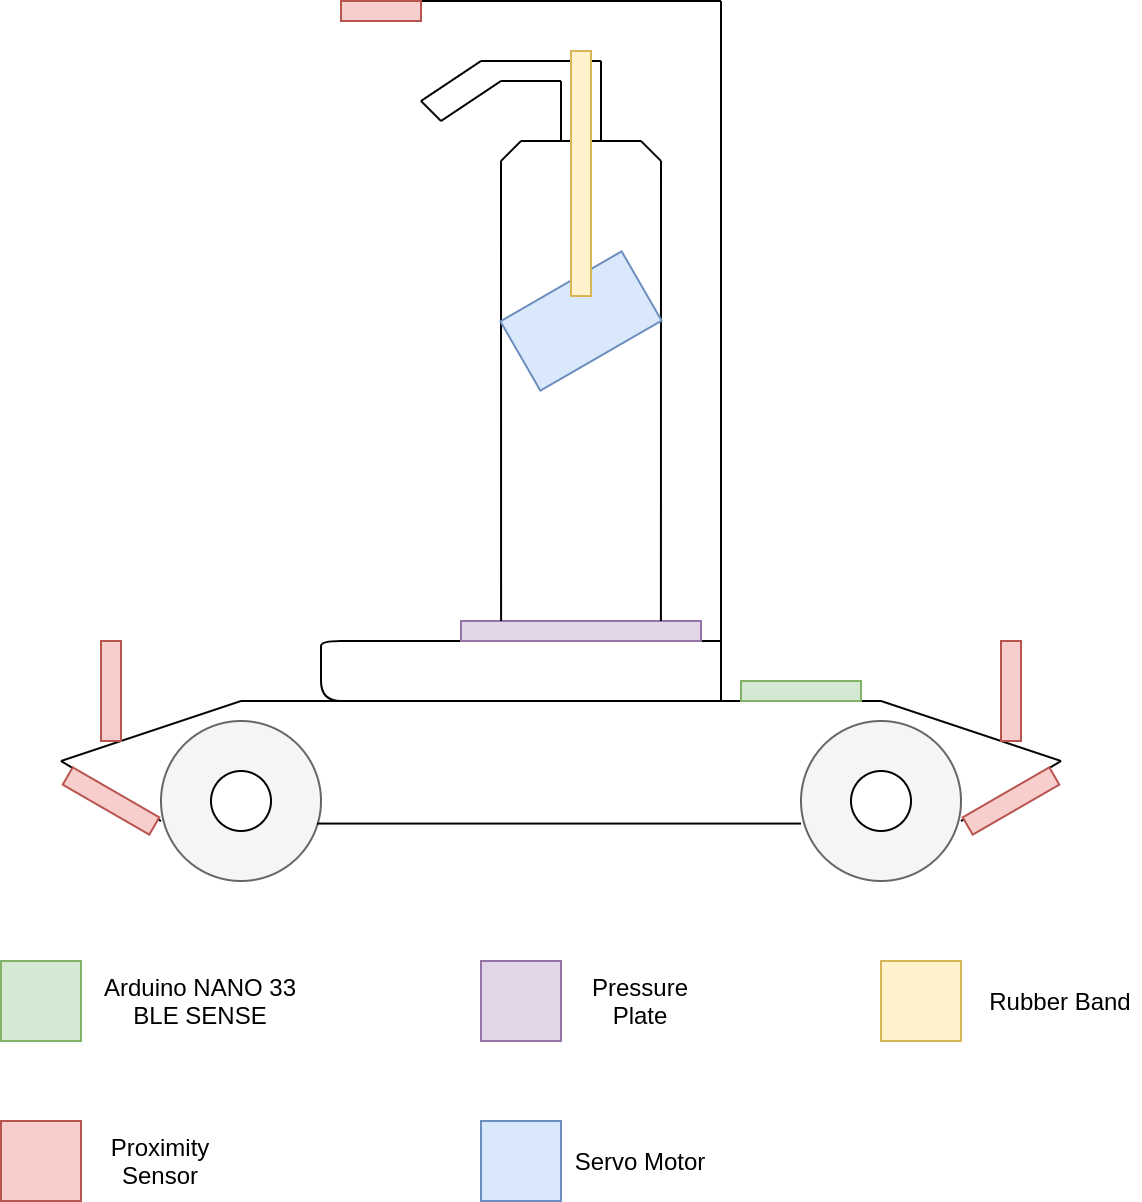
\includegraphics[width=\linewidth]{prototype-drawing.png}
	\caption{Prototype drawing of our vehicle}
	\label{ProtoDrawing}
\end{figure}

As the car would provide people with antibac, we naturally wanted the car to be able to drive on top of a table. That is why it had downpointing sensors, to be able to know when it would drive of an edge. However, after receiving the car from our professor, we quickly found, that the navigation system we would need to implement would be way too comprehensive, given the small timeframe of the assignment.\\ 

Throughout the project, the system went through several iterations, and as we met challenges along the way, the antibac idea was abandoned. The final design is illustrated in Figure \ref{final-design}. 

\begin{figure}[H]
	\centering
	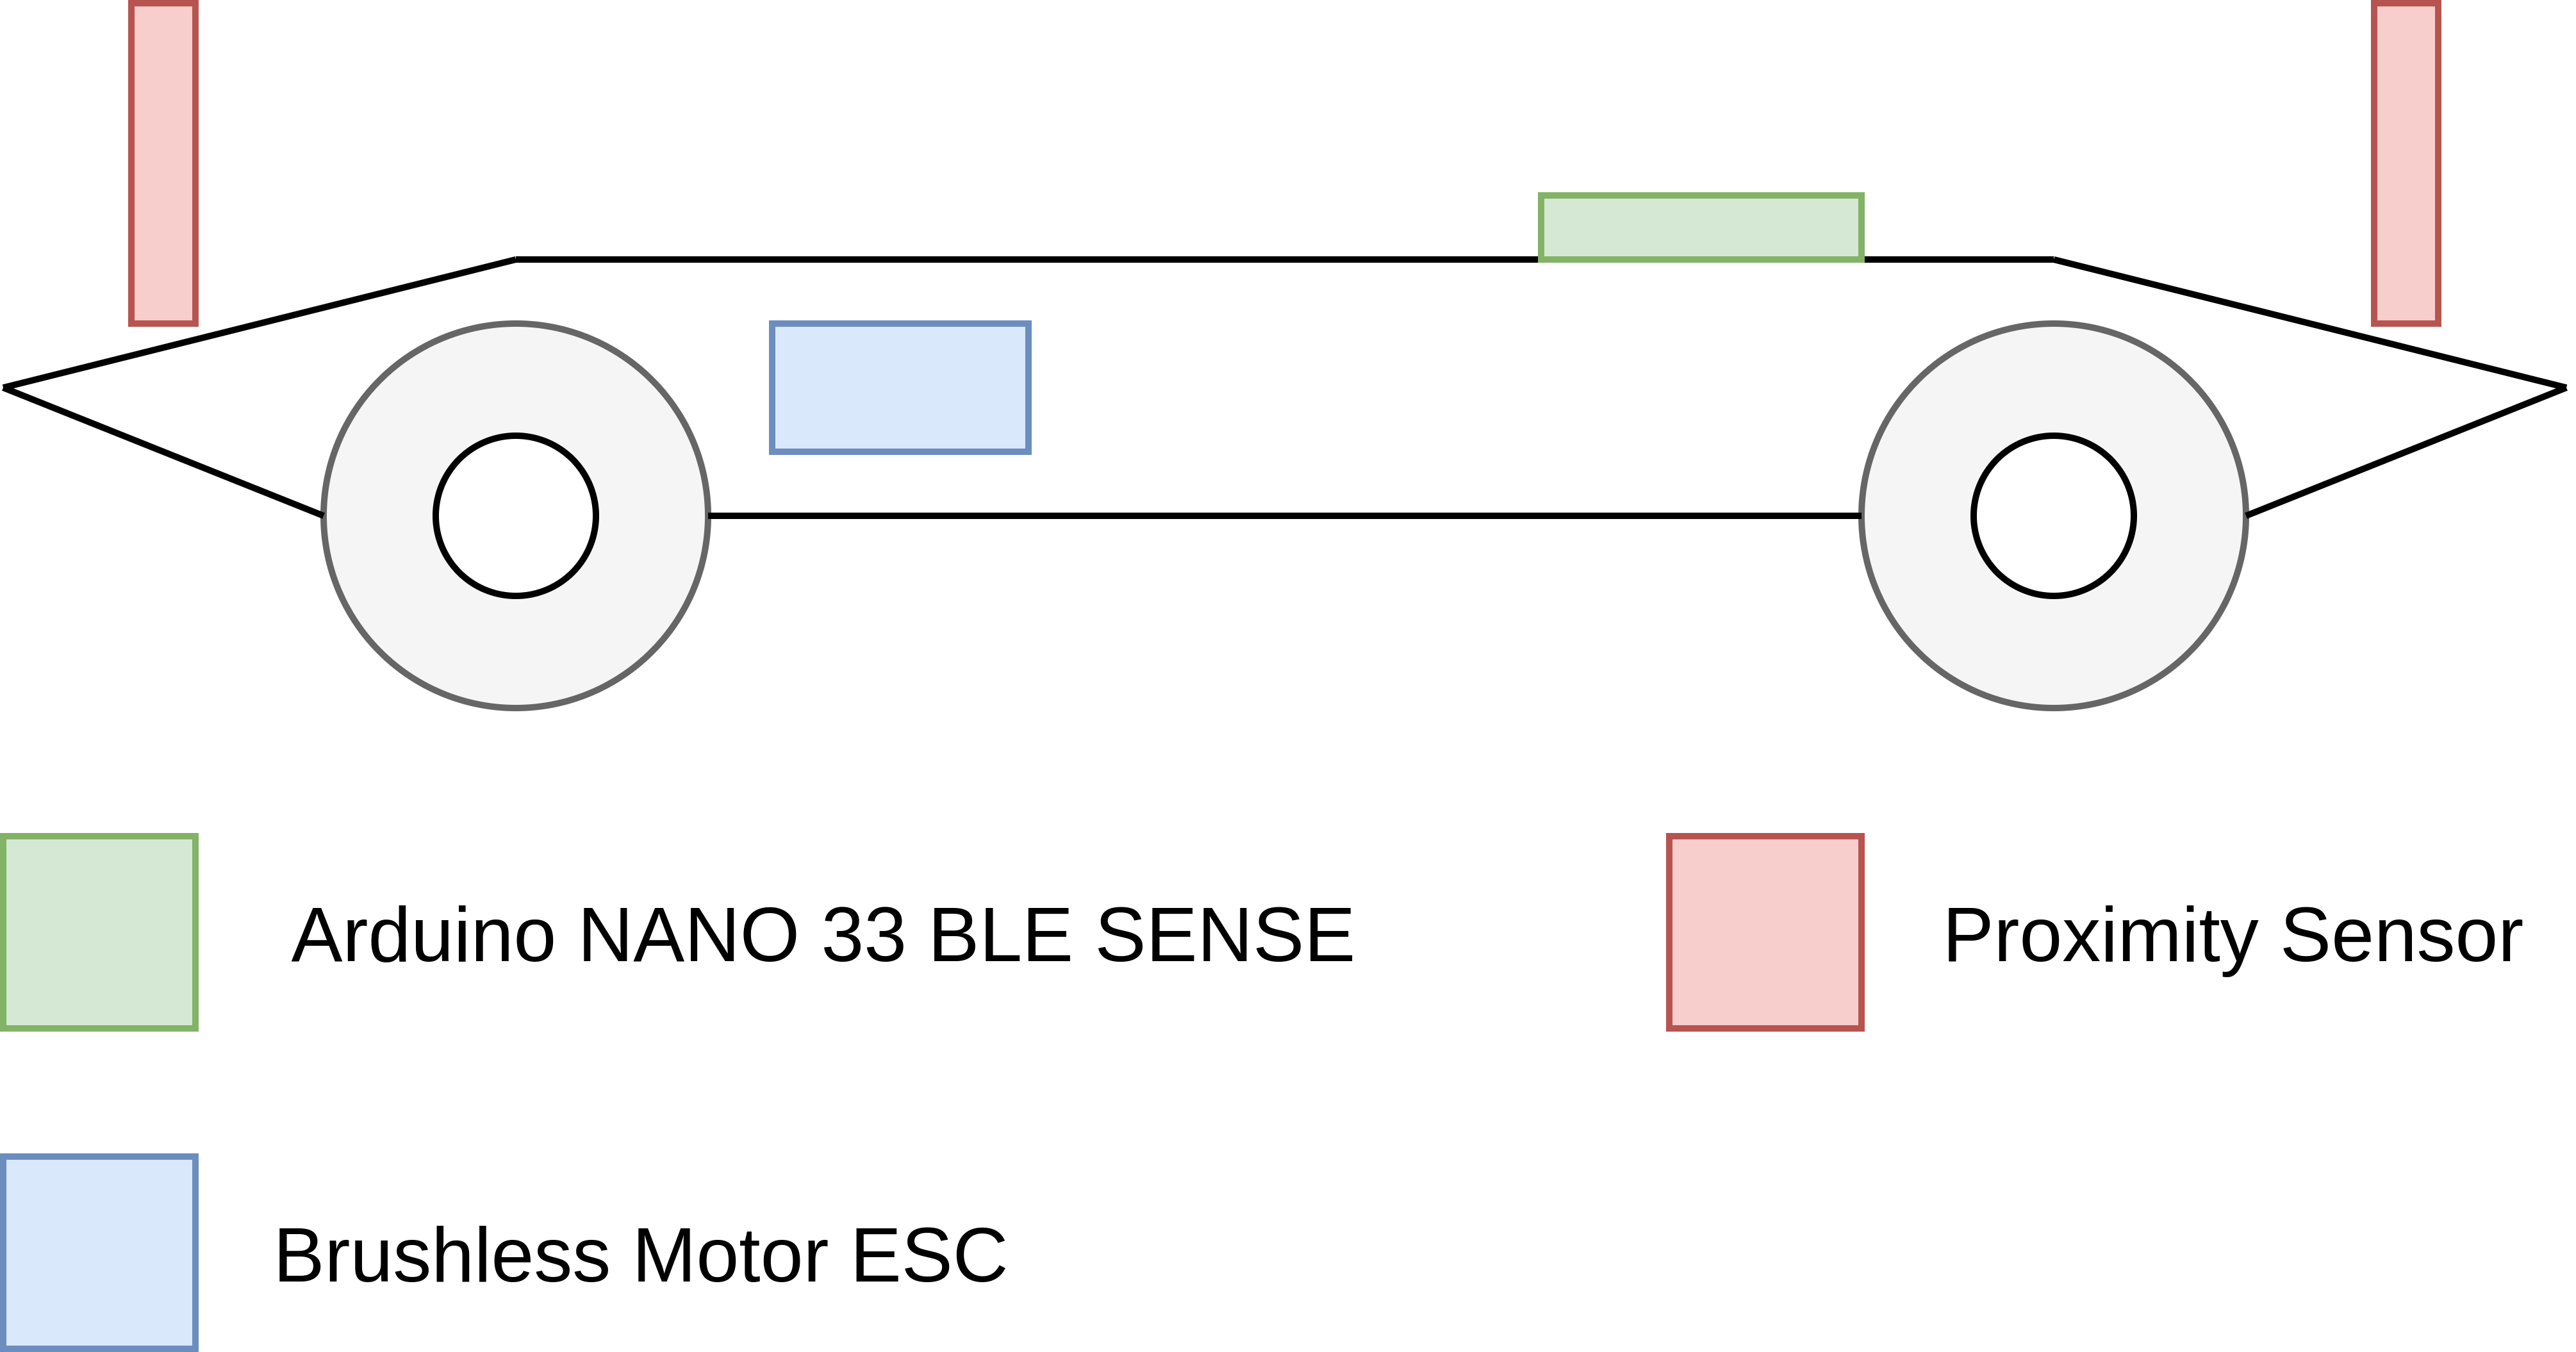
\includegraphics[width=\linewidth]{final-design.png}
    \caption{Missing Caption.}
	\label{final-design}
\end{figure}

\section{Technologies}

\subsection{The Ada Programming Language}
Ada was development for the American department of defence in the 80's in order to try and get a standard programming language for all of their projects. As its main use-case was intended to be on critical military systems, the language would be designed from ground up, to accomodate the creation of robust and safe software. This resulted in a language with strong typing, a strict compiler, and a syntax that is meant to improve the readability, resulting in a easier maintainability in large projects. Today Ada is still mostly used in the defence and aerospace sector, and is very suitable for embedded systems.\\


\subsection{Arduino Nano 33 BLE Sense}

The Arduino Nano 33 BLE Sense is a small microcontroller based on the nRF52840 microcontroller.
It comes with plenty of peripherals:
\begin{itemize}
  \item Bluetooth
  \item IMU
  \item Microphone
  \item Gesture/Light/Proximity detector
  \item Barometric pressure gauge
  \item Temperature and humidity gauge
\end{itemize}

\subsection{Servo Motors}
Usually, when programming Arduinos in C, one makes use of a library to control servo motors. However, as we were doing this in Ada, we would have to write our own library. Servo motors are controlled using a pulse width modulated signal (PWM). A PWM has a fixed period, where the amount of time the signal is high defines the signal. 

In the case of a servo motor, the fixed period is 20 milliseconds, and the signal must be high in a range between 1 and 2 milliseconds. Sending a 1.5 milliseconds high signal to a servo engine, is defined as the input for outputing neutral position. If we send a 1ms signal, the servo will move to the extreme left, and 2ms will output the extreme right. An illustration of this can be seen in Figure \ref{servo}.

\begin{figure}[H]
	\centering
	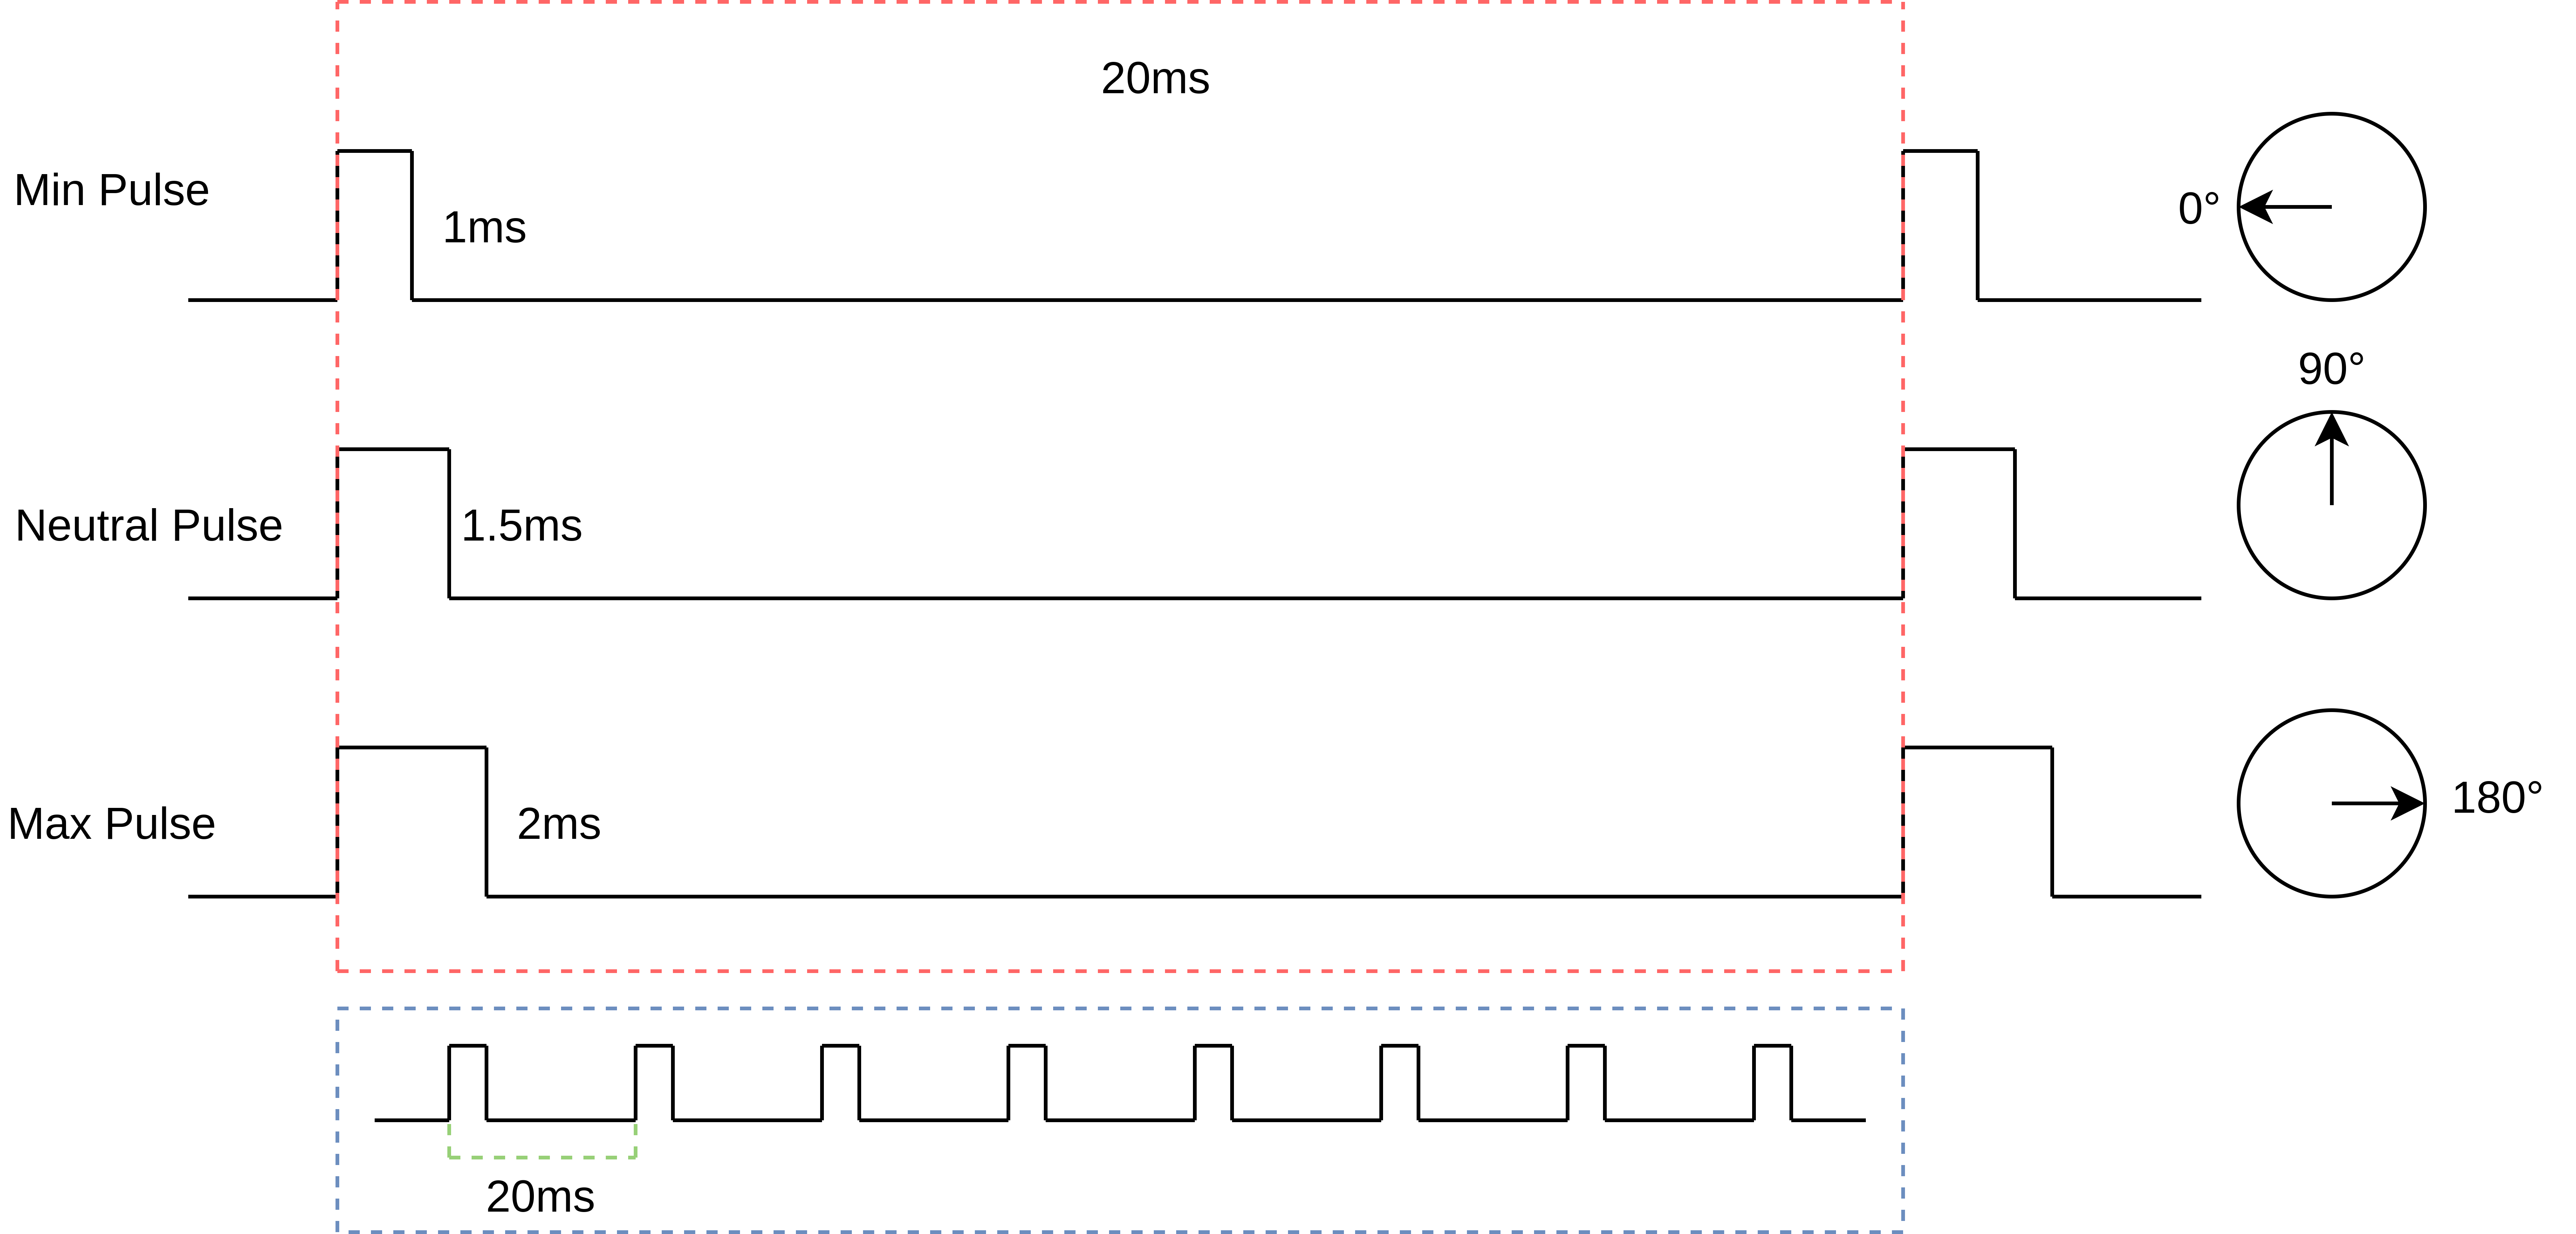
\includegraphics[width=\linewidth]{servo.png}
	\caption{Missing caption.}
	\label{servo}
\end{figure}

\subsection{Ultrasonic Sensors (HC-SR04)}
As the ultrasonic sensors has both input and output, they are a bit more complicated than the servo motors. They have a TRIG pin and an ECHO pin.\\ 

The TRIG is its input, where we send a signal letting it know that we want to perform a measurement. As illustrated in Figure \ref{ultrasonic-sensor}, it needs a sequence of a low signal for 2 microseconds, then a high signal for 10 microseconds. The ECHO pin responds with a signal, that when interpreted correctly, will tell us the distance to the closest object in the sensors facing direction. When the ECHO pin turns high, we initialize a timer which is active until the signal turns low. Dividing the time by 58 gives us the distance in centimetres.\\

\begin{figure}[H]
	\centering
	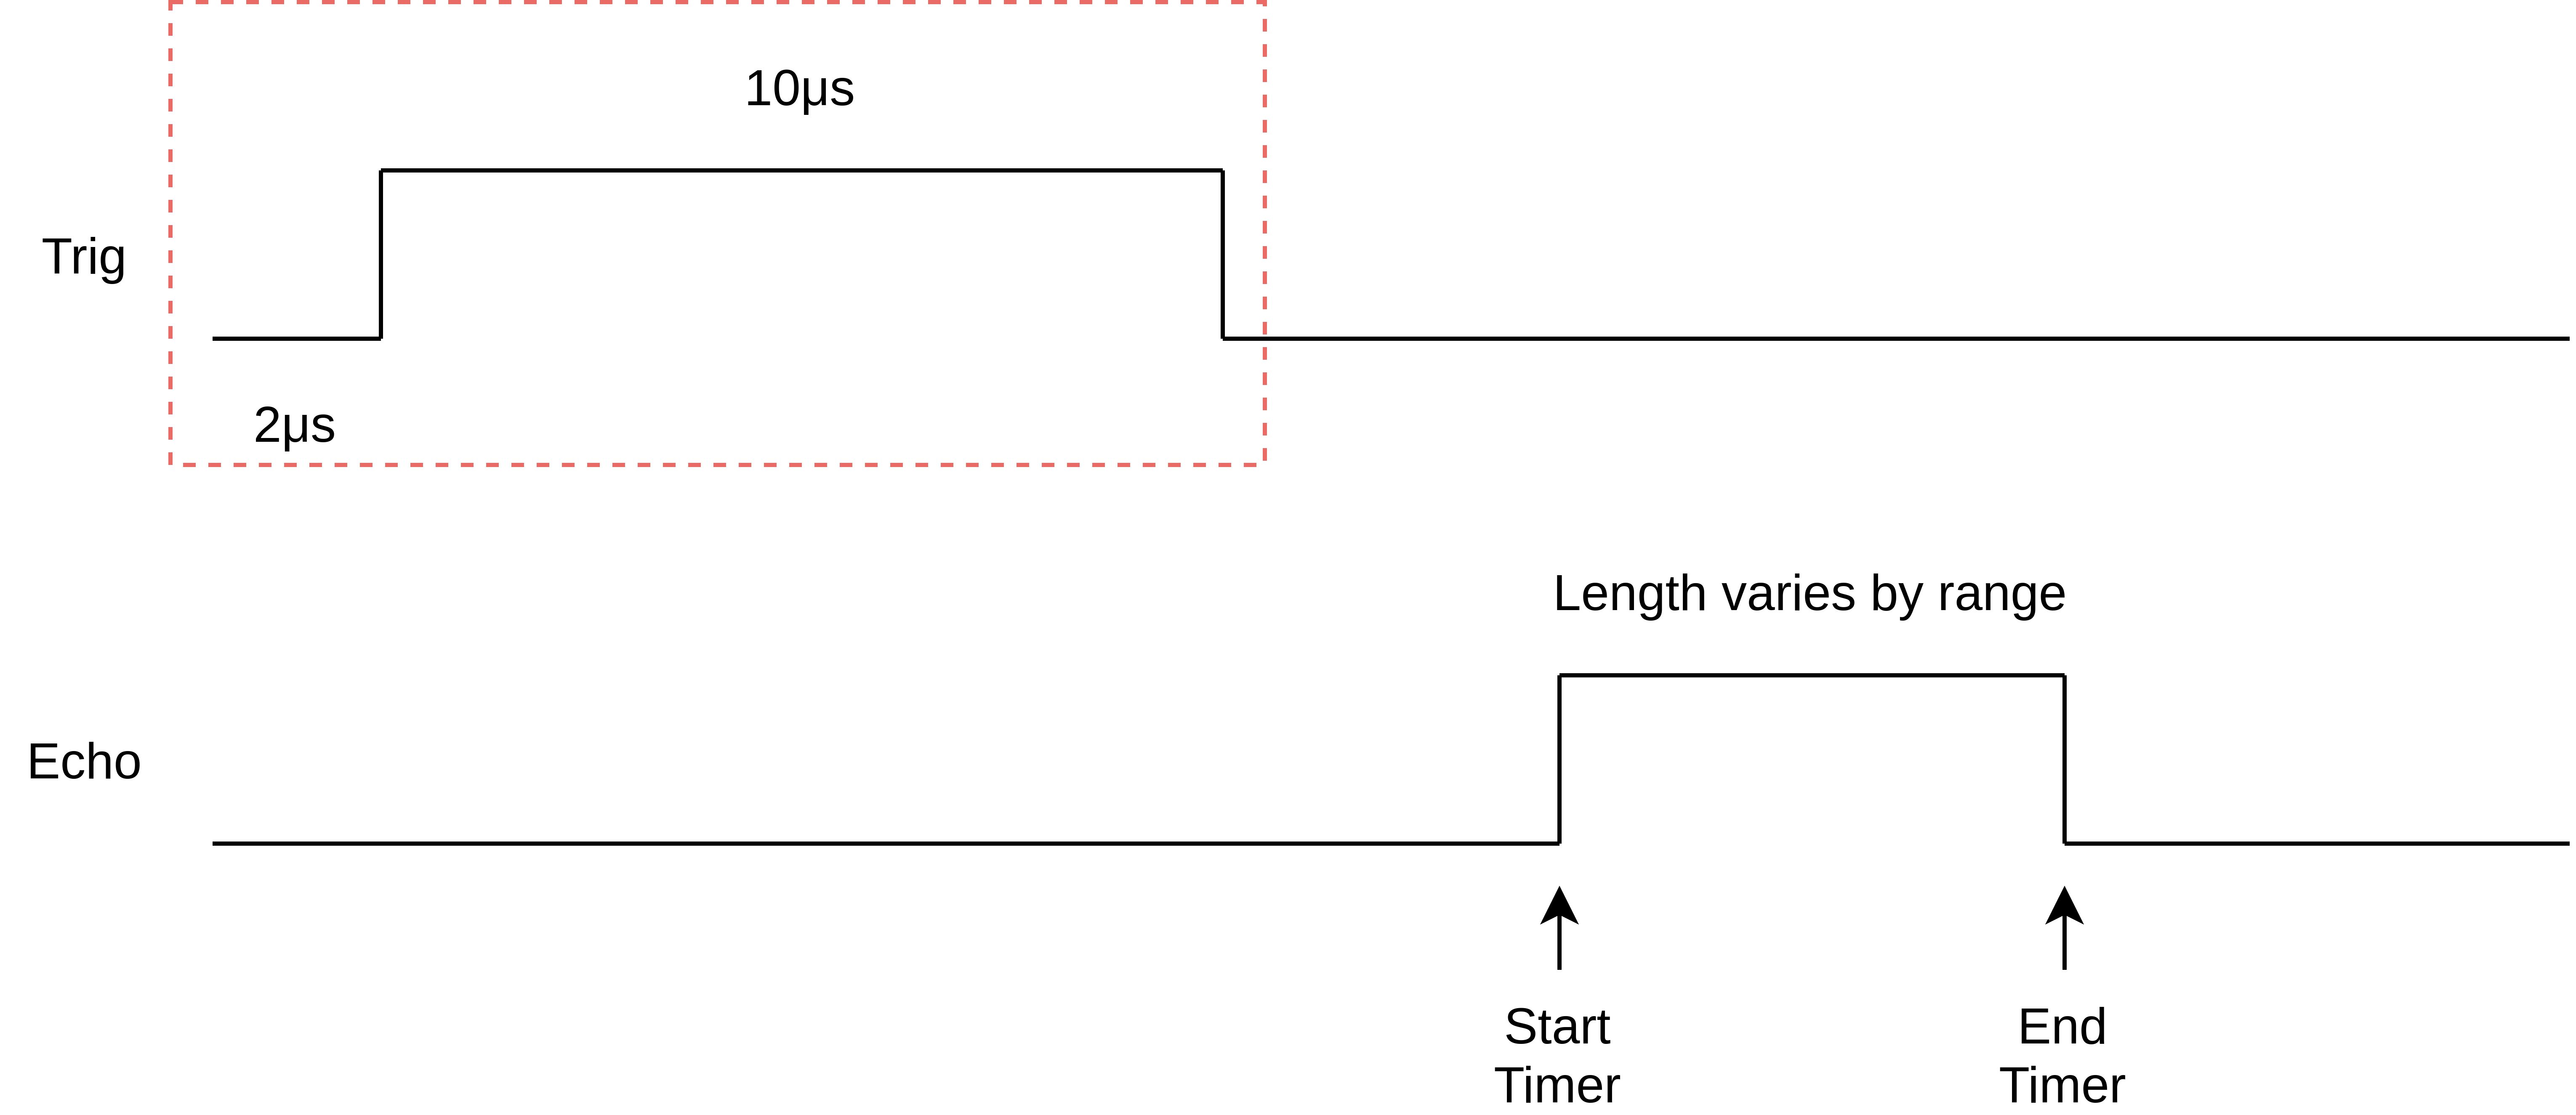
\includegraphics[width=\linewidth]{ultrasonic-sensor.png}
	\caption{Missing caption.}
	\label{ultrasonic-sensor}
\end{figure}


The signal.... ****Her må du skrive litt stian********




%Finn riktig navn på denne, pluss litt specs
\subsection{The Turnigy Trooper}
The Turnigy Trooper is the name of the car that our professor provided us with. It was originally a remote controlled car, but a lot is removed, so nothing but the chassis, motors and wheels remain.\\ 

A diagram of the components on the car can be seen in figure \ref{}

****Diagram av ECD, servo osv fra manual************


The servo motor for the steering is traditional one, which takes the PWM that was desribed previously.\\ 

The motor which will provide us with propulsion however, is actually a DC motor. Luckily for us, the ESC, provides a PWM interface for us, so that we can treat the motor as a fully rotating servo motor.\\ 

As in the case with regular servo motors, we send it a standard PWM signal, but in this case, the high time of the signal does not refer to a static deegree, but to the speed of rotation. As can be seen in figure \ref{esc}, a high signal of 1.5ms means that the motor will not rotate. If we send a 2ms signal it will rotate forward at the highest speed, and the opposite applies for 1ms. 

\begin{figure}[H]
	\centering
	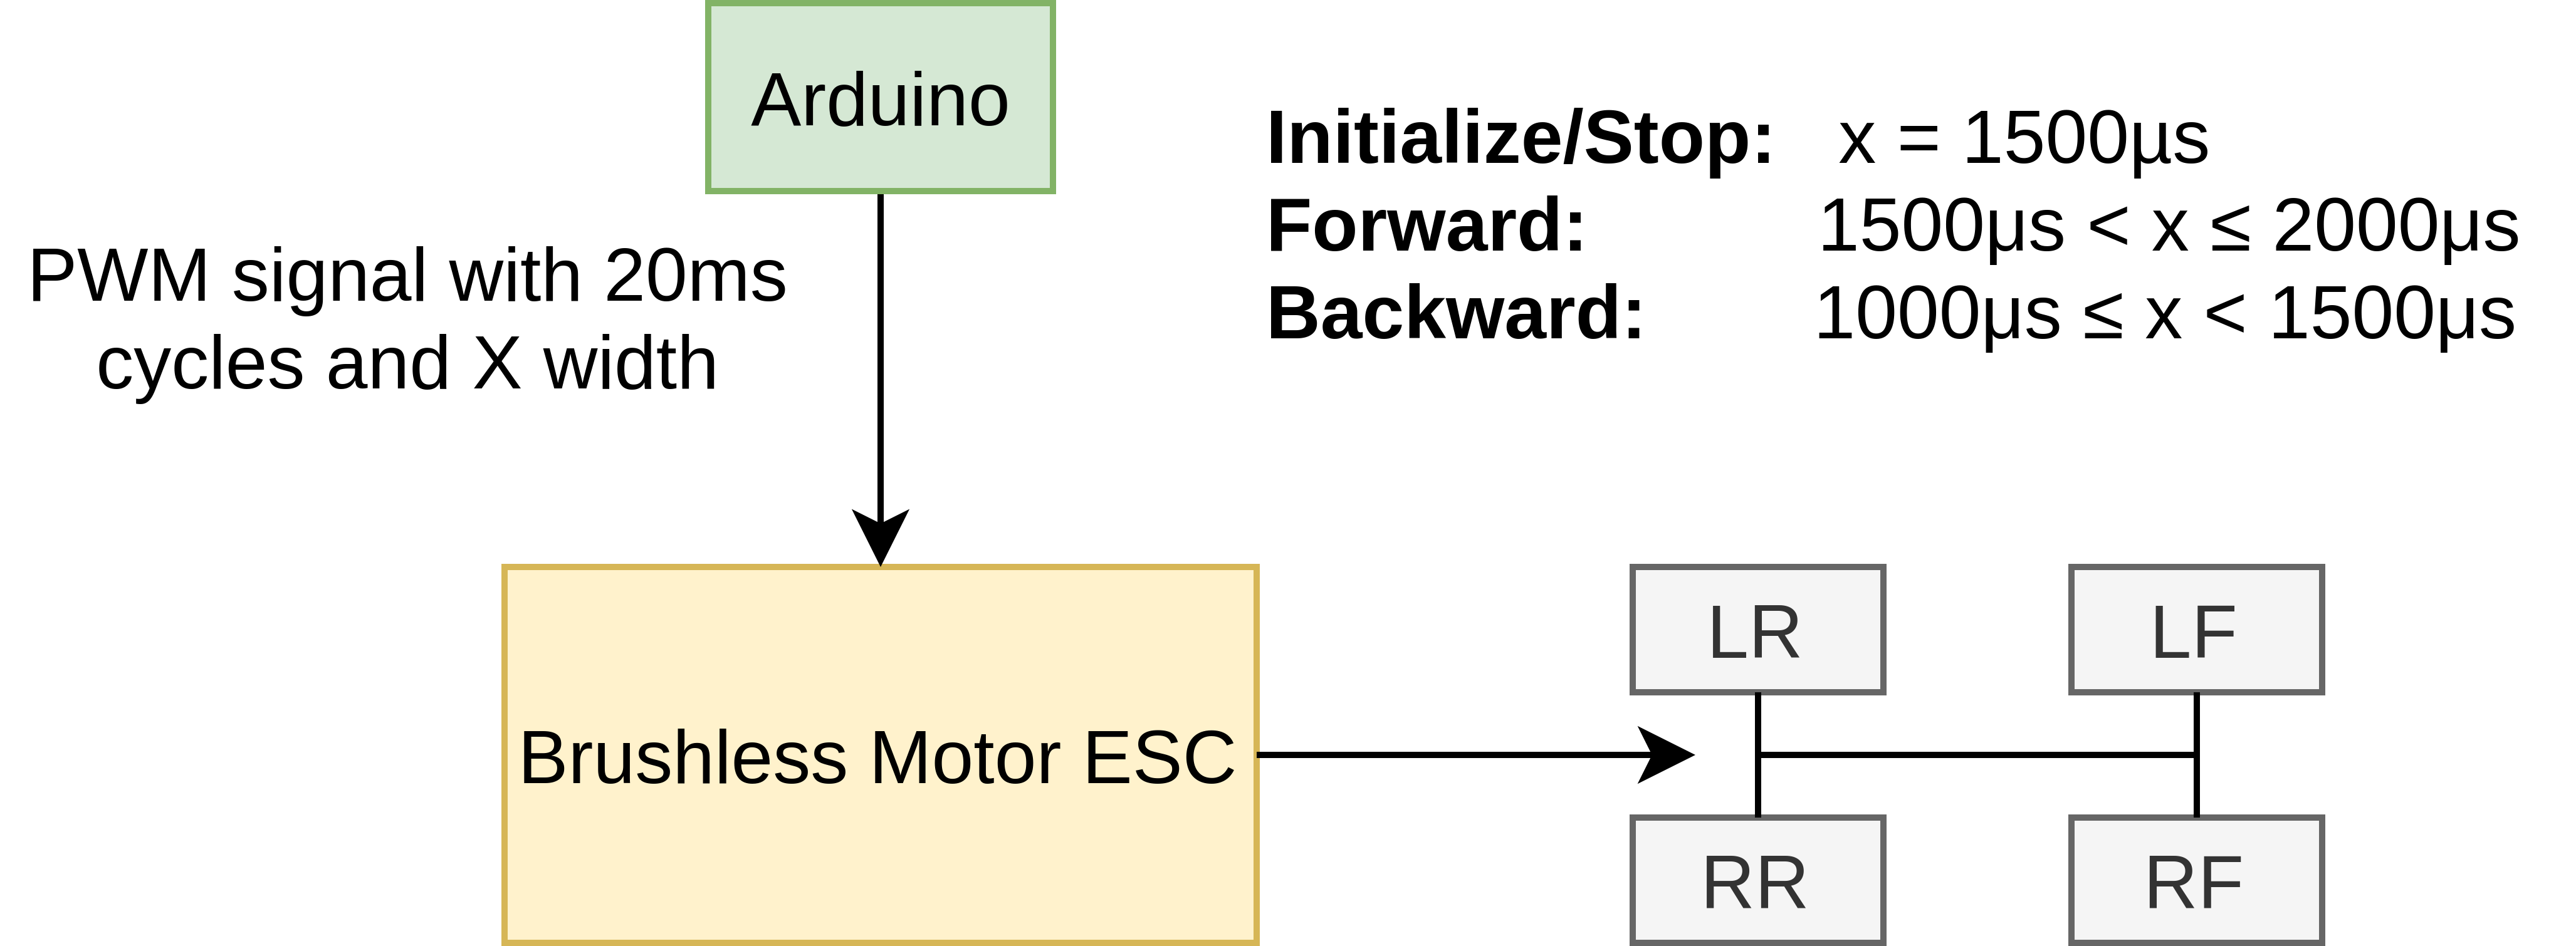
\includegraphics[width=\linewidth]{brushless-motor-esc.png}
	\caption{Block diagram of signal path from Arduino}
	\label{esc}
\end{figure}


The ESC in the Turnigy Trooper is also possible to program quite extensively, and after receiving the manual, we played around with the settings for a bit, before deciding that the default settings would suit us fine. 

\section{Toolchain \& Testing}
\subsection{Ada on the Arduino}
As we were told early on that almost noone had programmed Ada on the Nano, we knew early on that this would be a challenge. We didn't really know were to begin, until our assistant professor, Steven Bos, pointed us in the right direction. 

\subsubsection{Ada Drivers Library}

The \textit{Ada Drivers Library}, is a collection of drivers and examples for programming Ada on a wide range of microcontrollers, however the Arduino Nano was \textbf{not} one of them. However, as Steven Bos had discovered, it does provide drivers for the \textit{NRF52\_DK}. This board has the same CPU, \textit{Arm Cortex-M4} and a similar microcontroller as the Arduino Nano. Steven presented a working solution for a classical led blink example using this library, and after that we at least had a path to follow, as well as expanding on.\\ 

We knew that it would be quite a few hours of adjusting the existing drivers, to suit the Nano. In the hope of being able to contribute to the open-source community, we forked the \textit{Ada Drivers Library}
, and used their script to build basic board files for the Nano, based on our inputted specifications. 

\begin{figure}[H]
  \centering
  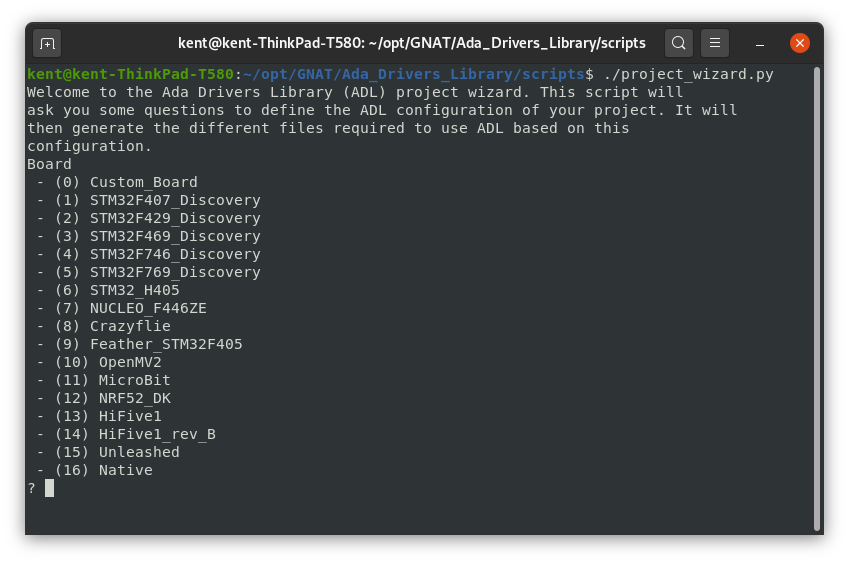
\includegraphics[width=\linewidth]{projectwizard.png}
  \caption{Screenshot of the project wizard from Ada Drivers Library}
  \label{projectWizard}
\end{figure}
\subsubsection{Ravenscar runtime Library}

When flashing a microcontroller with code, you also need to have a runtime library. As a microcontroller is limited in space, you usually won't include everything that the language normally offers.\\ 

For most of the microcontrollers in the \textit{Ada Drivers Library}, there exists three kinds:
\begin{itemize}
  \item{ZFP (Zero footprint library)}
  \item{Ravenscar SFP (Small footprint library)}
  \item{Ravenscar Full}
\end{itemize}

For the NRF52840, the only runtime library that was provided to us out of the box, was the ZFP. The ZFP has (as the name implies) almost none of the features we would need. The most crucial one being the ability to have multithreading (called tasks in Ada). As much of this course's theory is based around having several tasks, and how to schedule them etc, a sequential approach would not do.\\ 

In order to have access to the Ravenscar full library, we cloned BB-runtimes from Github, and used a script they provide in order to build it. This proved a tedious task, and there were quite a few errors within the script that had actually already been fixed by the developers, but not released at that time.\\ 
%Er dette riktig forklaring????? 
Luckily for us, this eventually worked out okay. The ravenscar library still has its limitations which would change the way in which we structured our software. For instance, it does not allow entry points into tasks. This means that we would not have access to dynamic tasking, and that all tasks would have to be created statically. It also meant that we would not (without extreme difficulty) be able to take advantage of the multiple core processor on the Nano.\\

\subsection{Flashing the Arduino}

After getting our software toolchain together, we started trying to flash our Arduino with a blinkin test. As we had'nt received the JLink debugger yet, we wanted to see if this was possible to accomplish using only USB. After spending way too many hours on this, we found that this would not be feasible.\\ 

When we received the JLink debugger, we would unfortunately also have to wait for a 3D-printed clamp holder, as the soldering on the Nano had proved to be quite unstable for some of the other students. Our eagerness and impatiance luckily drove us to try and flash the Nano, whilst holding wires to the pins on the Nano by Hand. This took a lot of trial and error, but eventually some of the members of the group developed great skills for this technique, as can be seen in the picture below:

********Bilde av flashing med manuell holding av ledninger******************

When we finally received the clamp holder a few weeks later, flashing turned into a dream, and we could with much greater ease debug our program, as it no longer required someone manually holding the wires in place during runtime. 


%Finne på bedre tittel.
%Vil du fylle inn litt om pins her Tarald?
\subsubsection{Our Arduino library}

As mentioned, we built source files for our own drivers for the Arduino, using the scripts provided by the \textit{Ada Drivers Library}. Most of the files required only small changes, but the pin layouts are quite different on the Arduino compared to the NRF52\_DK. 

The nRF52840 has two ports, P0 has 32 pins while P1 has 16 pins.\\ 
We found the P1 base address for the nRF52840 seen on page 23 in the datasheet \cite{NRF52840}. Without it we were only able to use the pins with P0 seen on figure \ref{pinlayout}. After adding the base address to our Drivers Library and the option to chose between 0 and 47 pin number we were able to make all the pins function.

We also wanted to include the ability for analog writes and interrupts, but this proved to be overly complicated and timeconsuming to justify prioritization. More on this later. 

As the code is quite extensive, we have chosen not to include it in the appendices, but our fork of the \textit{Ada Drivers Library} can be seen on \href{https://github.com/Stykk-Gruppen/Ada_Drivers_Library}{GitHub}.

\subsection{Minimum working examples}

During the difficulties of flashing the Arduino, we spent our spare time writing both the full program, but also creating small testing suites. This would help us more efficiently test all the components, and how we interfaced with them, in a limited environment.\\ 

This helped us find quite a few bugs early on, as well as figuring out what would, and would not work.\\

For instance, the Ada Drivers Library has a servo motor example using analog write and interrupts. We initially tried doing it this way, to ensure steady PWMs for the servo motors, but as mentioned this proved to be much harder than anticipated. Because of our approach of test early, fail early, we were able to develop workarounds for this at an early stage.\\ 

We have developed testing projects to test the servos and the ultrasonic sensors. To test every pin on the board, we developed a blinking example, turning every pin on and off. The code for these tests can be found in our GitHub repository.

\section{Implementation}

\subsection{Hardware}
The car has a 7.4V lithium battery, it powers the ESC and the motor. We can power the Arduino with the lithium battery, but the sensors require 5V. We use a converter from Henning and a 9V alkaline battery to power the two sensors.

The bsensors have two connections to the Arduino, in and out while the ESC has a single connection.

In Figure \ref{Hardware} we have drawn our wire setup, with common ground for both power sources.
\begin{figure}[H]
  \centering
  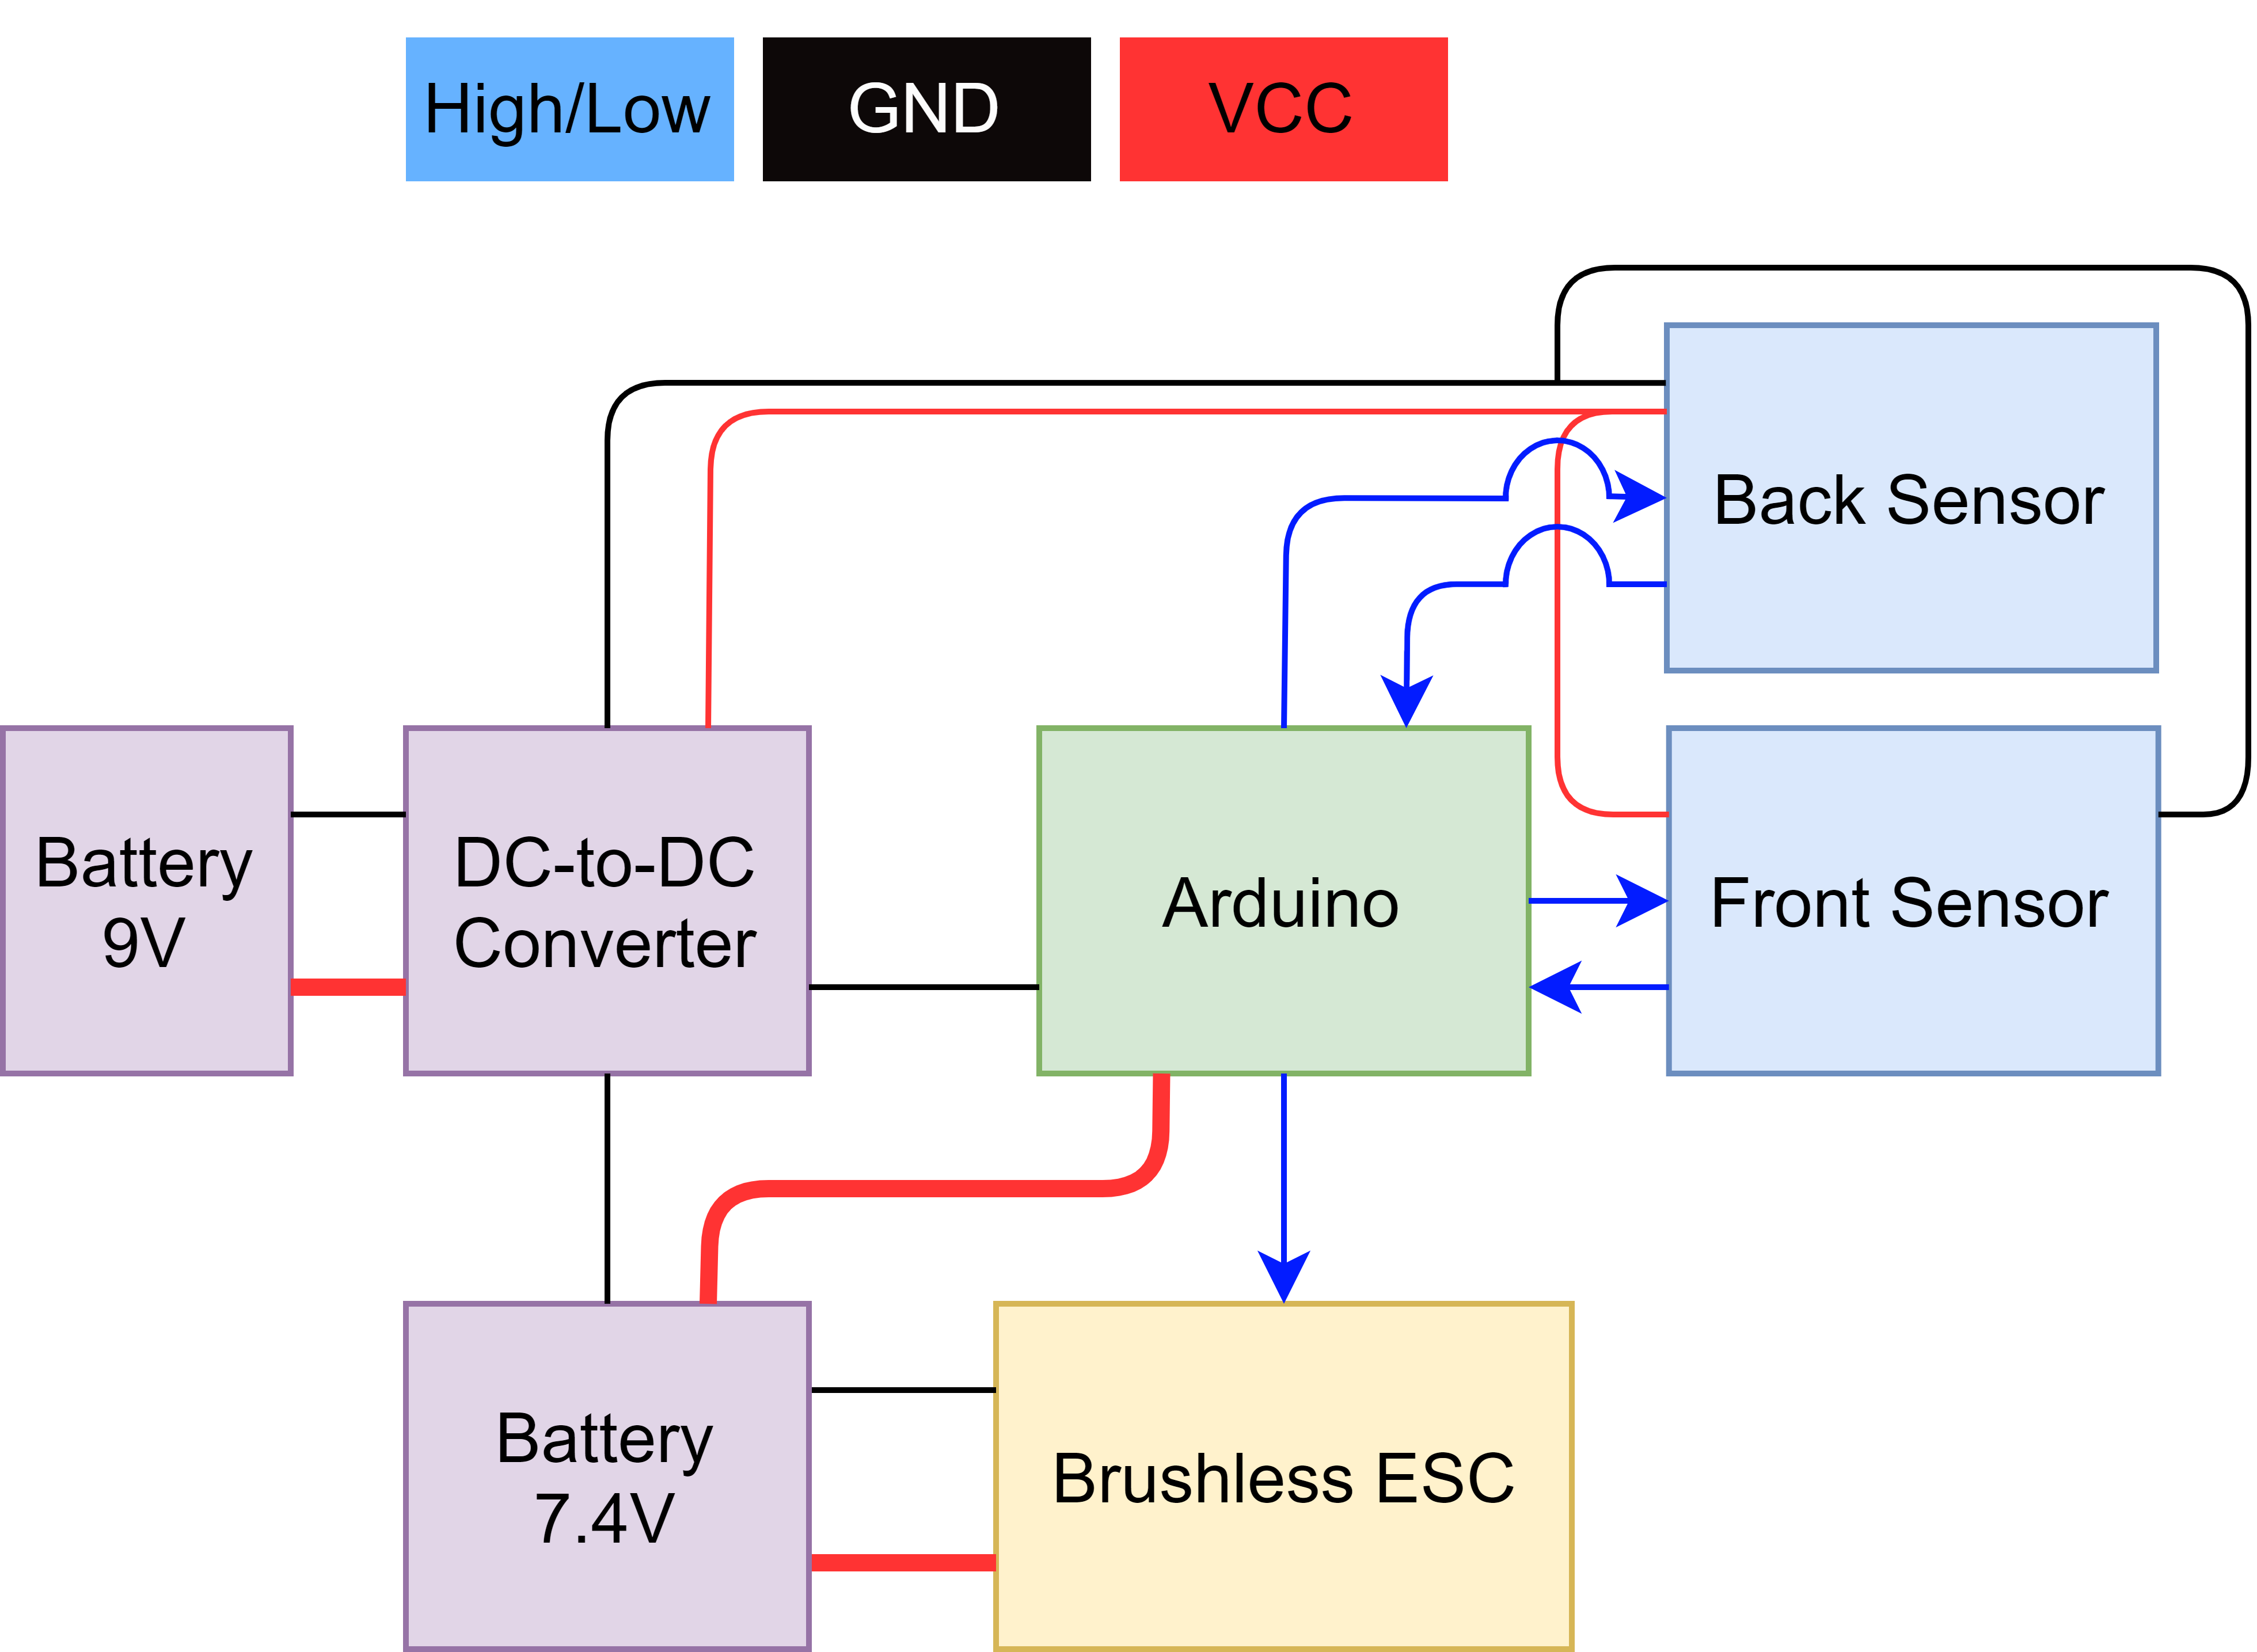
\includegraphics[width=\linewidth]{hardware.png}
  \caption{Block diagram of our hardware wiring}
  \label{Hardware}
\end{figure}

\subsection{Software}

\subsubsection{Architecture}
The system architecutre is illustrated in Figure \ref{SystemArchBlock}. The Distance Sensor Controller keeps a hold of the ultrasonic sensors. It operates them all in one task, reading the values sequentially and stores them in the controller. The servo controller was initially made to control the steering servo, the ESC and the two servos used in operating the dispenser. As the project deadling got closer, we had to remove the three servos and were left with the ESC. Even though the Brushless Motor ESC is technically not a servo, it uses the same operating signals as the other servos. At the time it made sense to fit it in with the others under the same controller.\\

The main component is the Vehicle controller. It reads the sensor values from the Distance Sensor Controller and uses them to calculate the next sate logic. Each state writes their own unique values to the Servo Controller. These values indicates the signals sent to the ESC, altering its speed.

\begin{figure}[H]
	\centering
	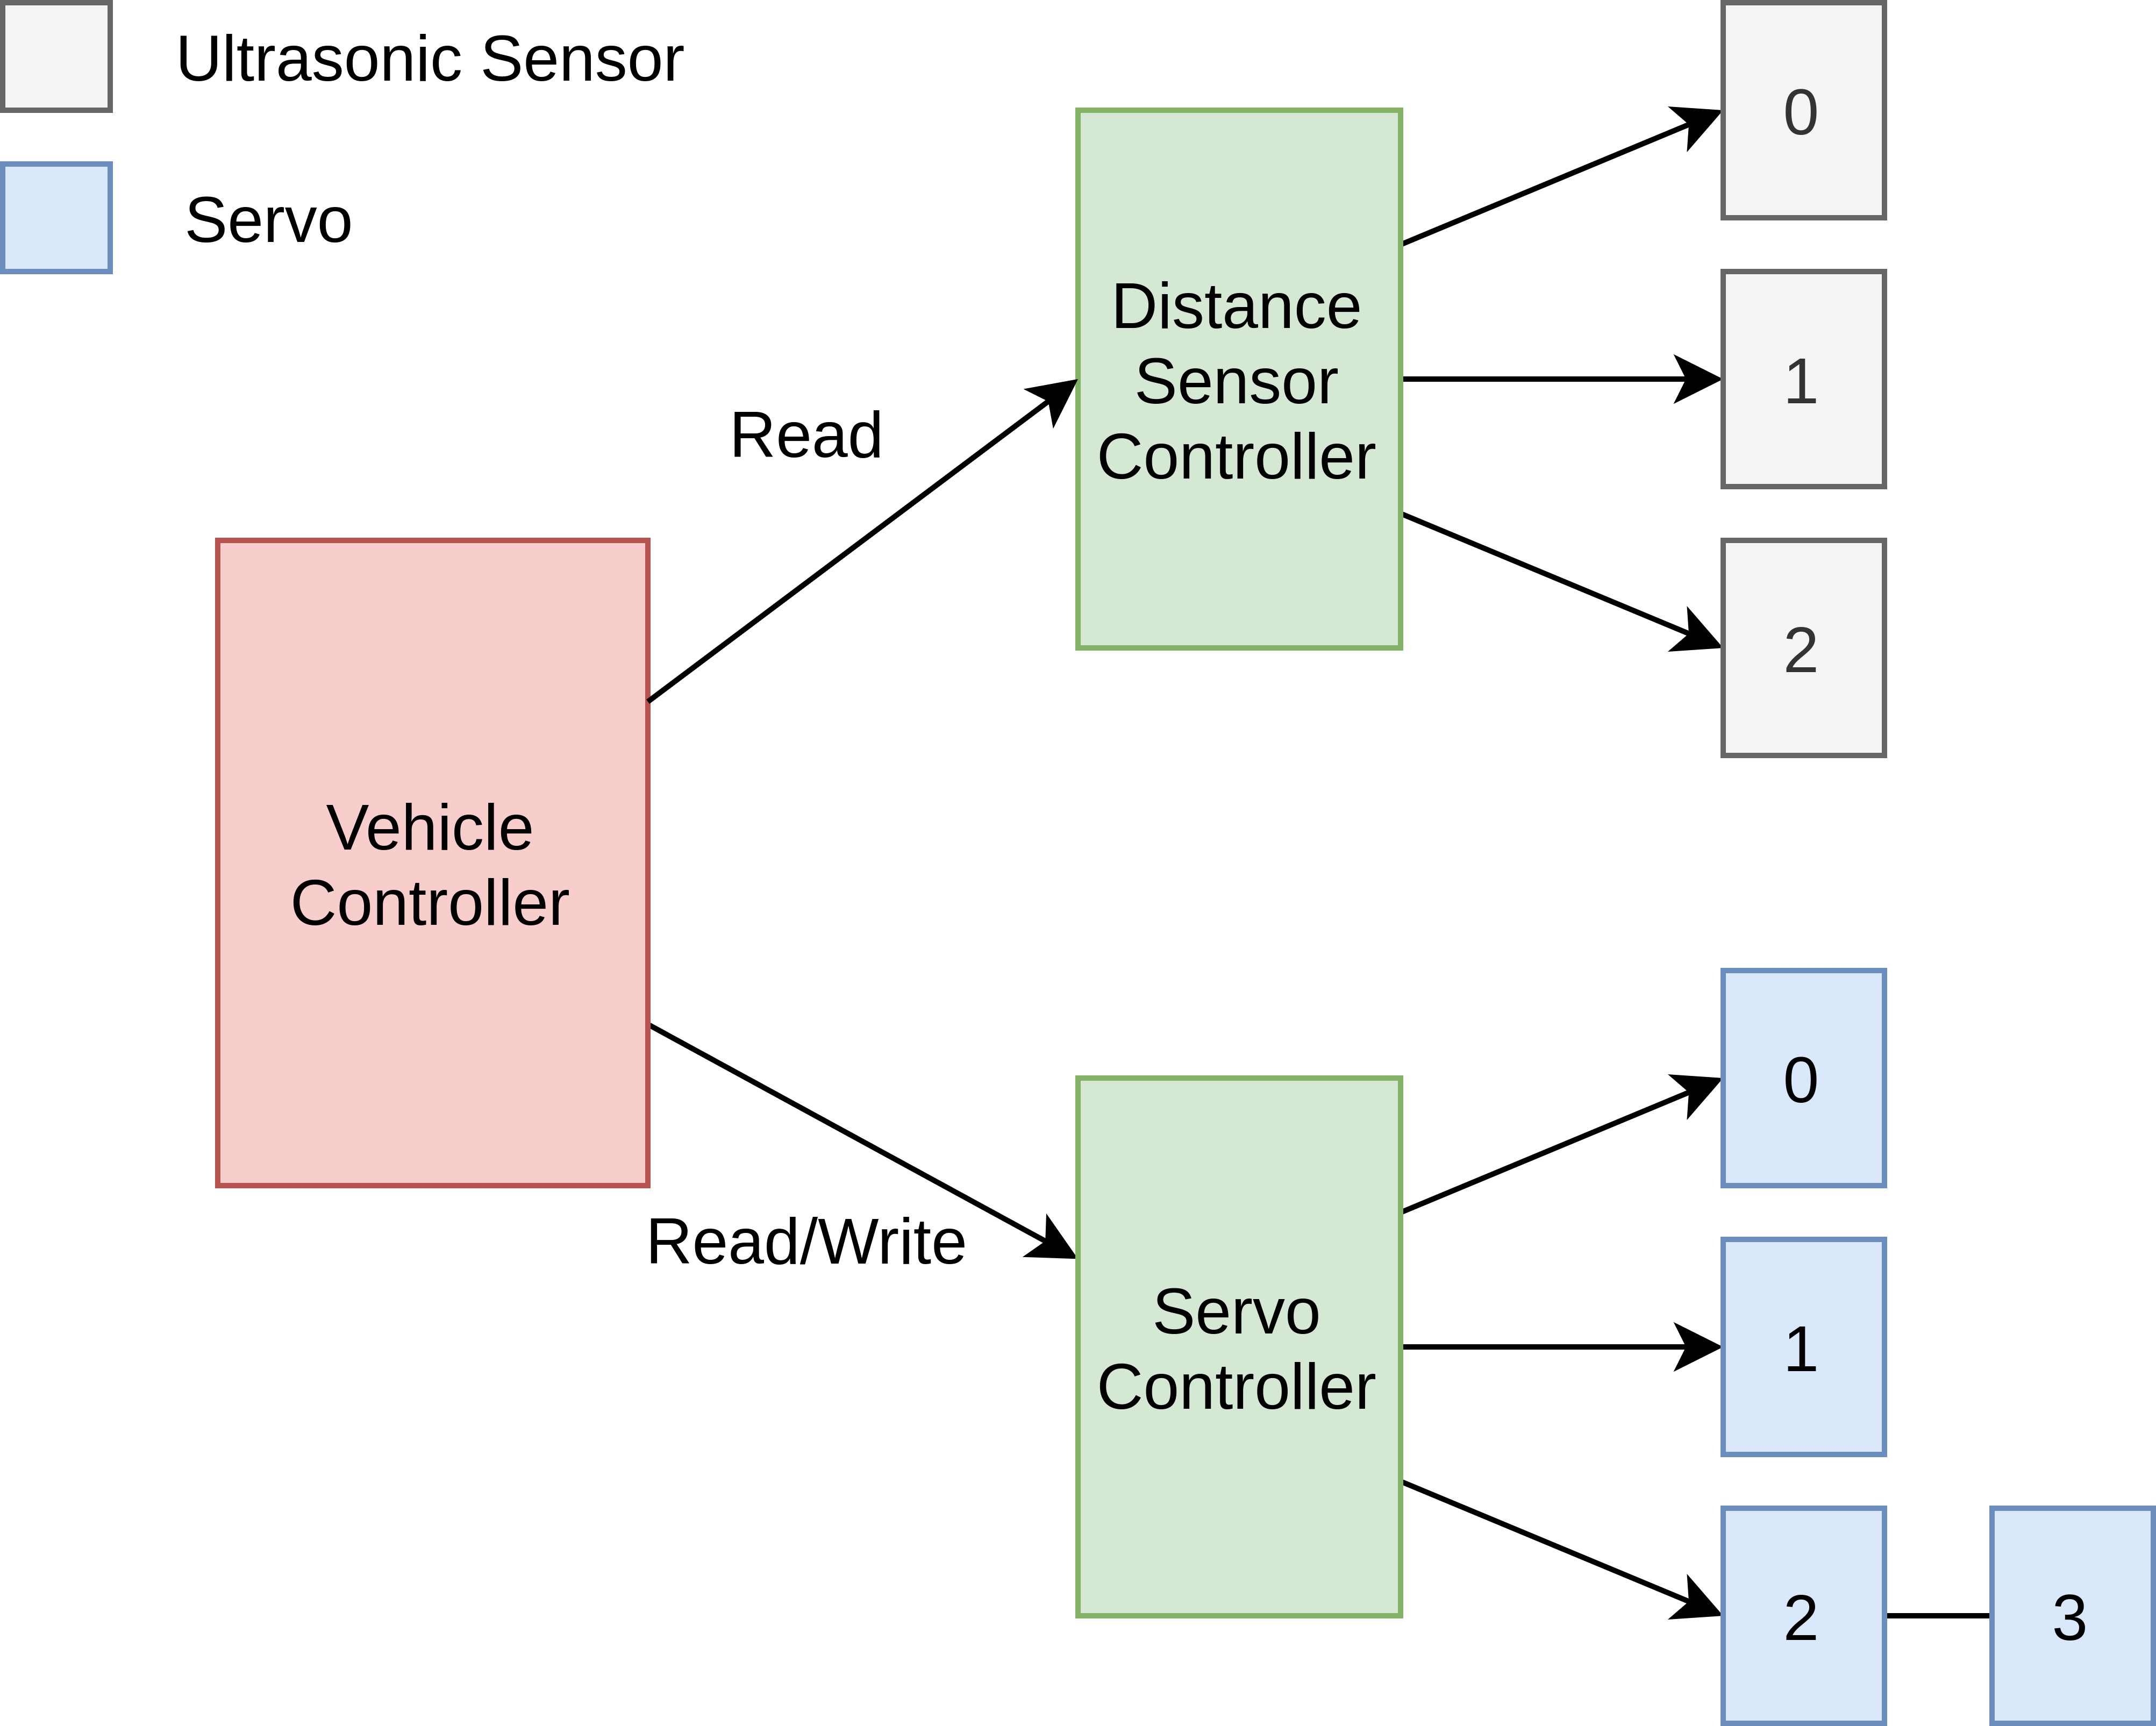
\includegraphics[width=\linewidth]{system-architecture.png}
	\caption{Block diagram of our system architecture}
	\label{SystemArchBlock}
\end{figure}

\subsubsection{Scheduling}

\section{Various problems we've encountered along the way}
In the list below are some problems we have encountered during our development phase from 17.09.2020 - 23.10.2020. Most of these issues have occured using Linux, it is stated otherwise.

\begin{itemize}
	\item Flashing to the Arduino board without a debugging probe might be impossible.

	\item After installing software for the Segger J-Link debugger from their official webpage, a new .rules file for the debugger appears in $/etc/udev/rules.d$ containing the necessary information for the debugger to be found by $pyocd\ list$. This has only been successful with one of our computers. A workaround is to run pyocd with sudo privileges.

	\item Including unused libraries in the Ada source-code makes the arduino crash under run-time.

	\item When trying to flash to the board without having the cables soldered, errors in the list below have appeared as a consequence of unstable hands.
		\begin{itemize}
			\item Unable to start CPU core.
			\item Target System has no power.
            \item Unspecified Error.
            \item J-Link is already open.
		\end{itemize}

	\item Including Arduino\_Nano\_33\_Ble\_Sense.Time makes the microcontroller crash in real time. --ref til Debug lstlisting i appendix--

	\item Only Digital I/O works. Possibly because Analog relies on interrupt/timers which seem broken in our drivers or runtime.

	\item Generating a pulse accepted by the servos and ultrasonic sensor is more challenging than setting pins to low/high and using a delay.

	\item Using a copied bb-runtime library will not work correctly on other computers under debugging. They must be generated on the debugging enviorment.

\end{itemize}

\section{Final Product}
To sum it up, the final product is a car, that will drive forwards and backwards, and avoid hitting walls. 

\begin{figure}[H]
	\centering
	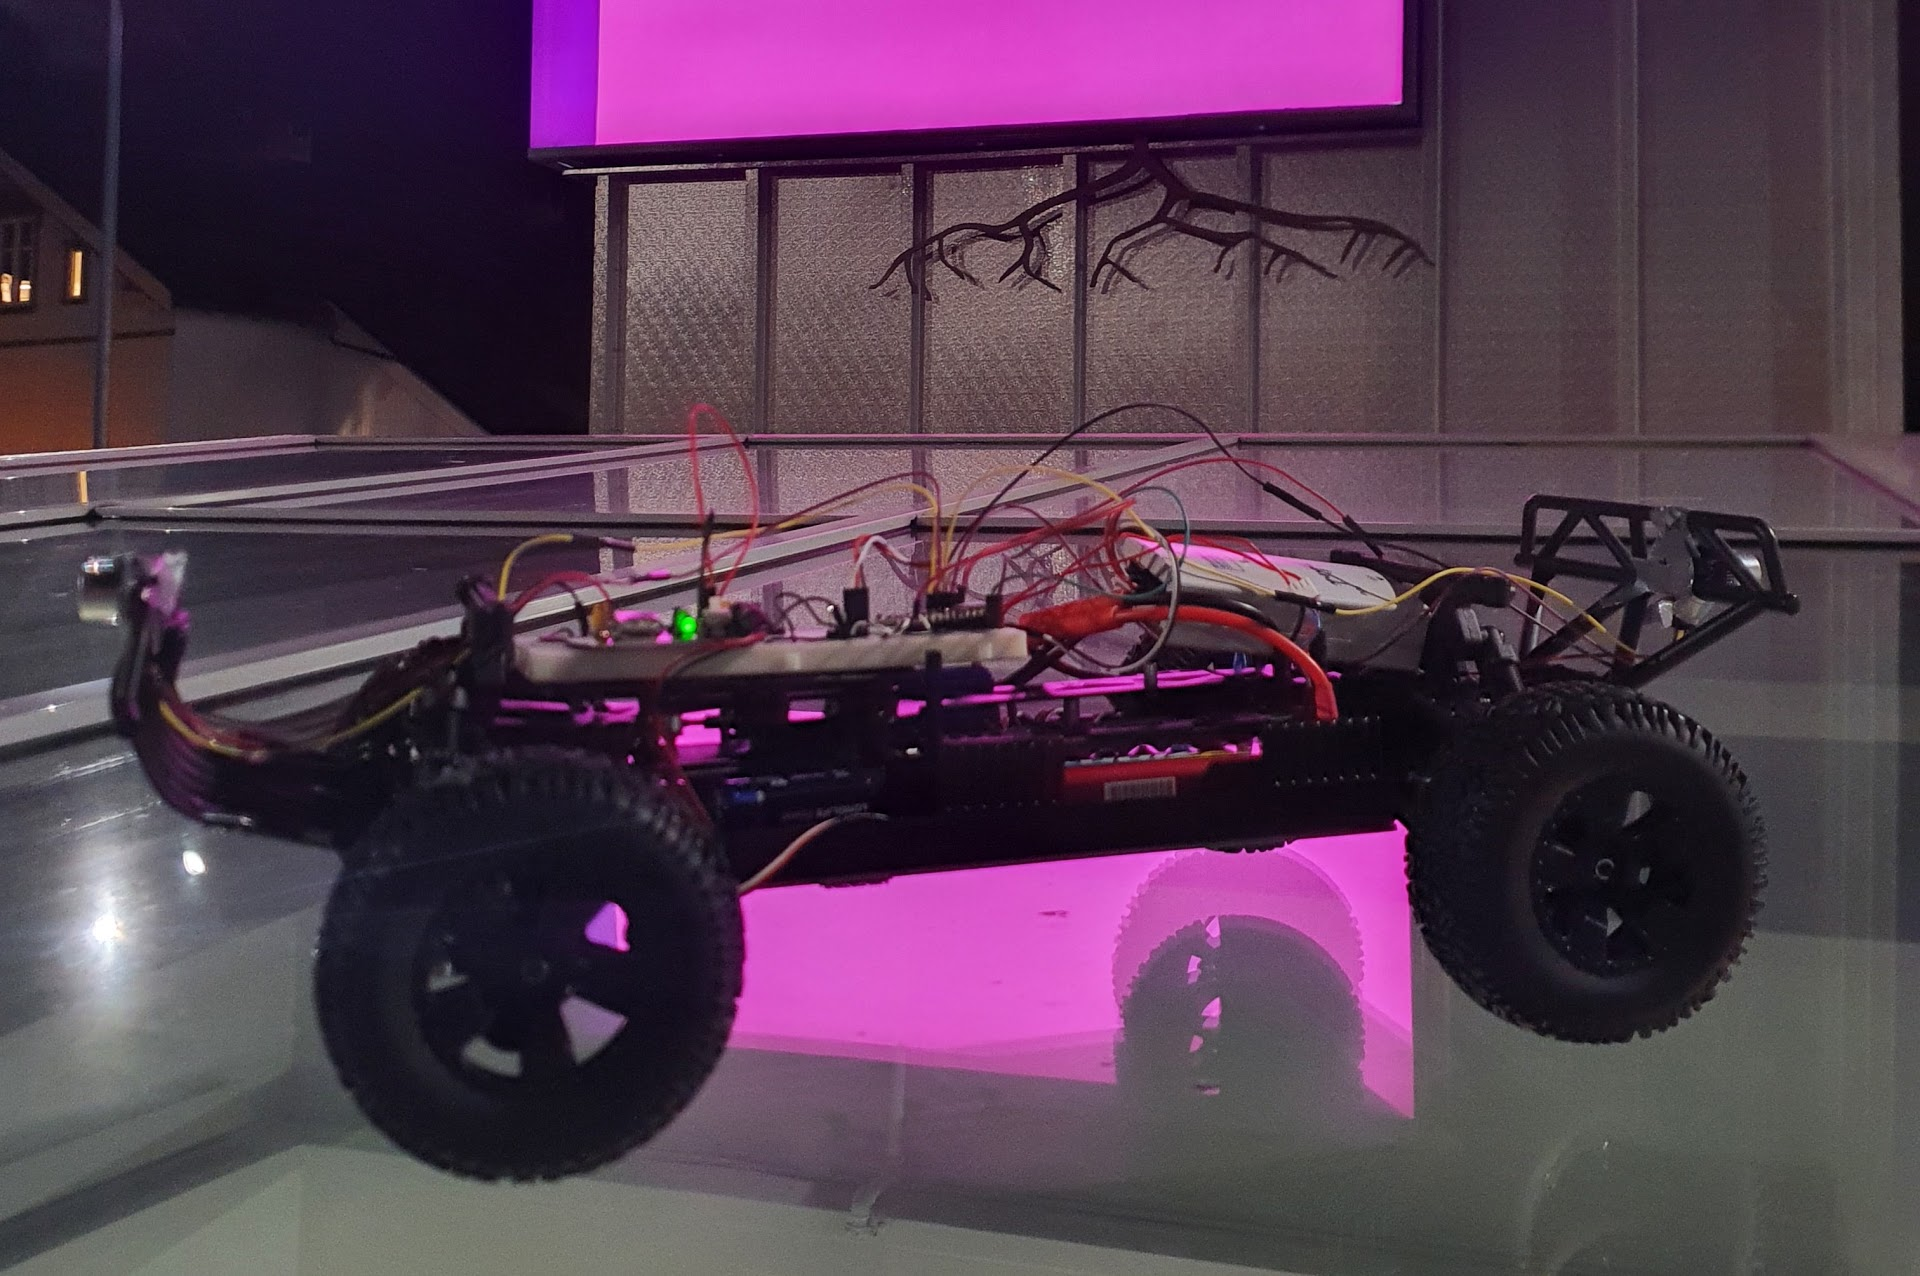
\includegraphics[width=\linewidth]{showcase.png}
	\caption{Missing caption.}
	\label{showcase}
\end{figure}

\section{Conclusion}

The purpose of this assigment was to try and implement the theory relating to real-time systems in practice, in order to better understand it. In spite of the challenges along the way, and how we had to downscale the project several times, we would still say that this goal was accomplished.\\

One can read about the difficulty of making a system meet all its deadlines, how scheduling works and what happens when a thread is starving, nothing can beat the feeling of actually experiencing it. As mentioned, we had several tasks that did'nt deliver the output we expected, and many times this was due to the task not getting any time on the CPU. That is a powerful experience.\\ 

Learning to program in Ada along the way, as well as building the the ravenscar run-time library and the library for the NRF52840, was great, is guaranteed to prove very useful knowledge in the future.\\ 

\newpage
%Referanse
\nocite{*}
\bibliographystyle{plain}
\bibliography{ref}
\addcontentsline{toc}{section}{References}

\newpage
\section{Appendices}

\lstset{frame=tb,
extendedchars = true,
texcl=true,
  language=Ada,
  aboveskip=3mm,
  belowskip=3mm,
  showstringspaces=false,
  columns=flexible,
  basicstyle={\small\ttfamily},
  numbers=none,
  numberstyle=\tiny\color{gray},
  keywordstyle=\color{black},
  commentstyle=\color{dkgreen},
  stringstyle=\color{mauve},
  breaklines=true,
  breakatwhitespace=true,
  tabsize=3
}

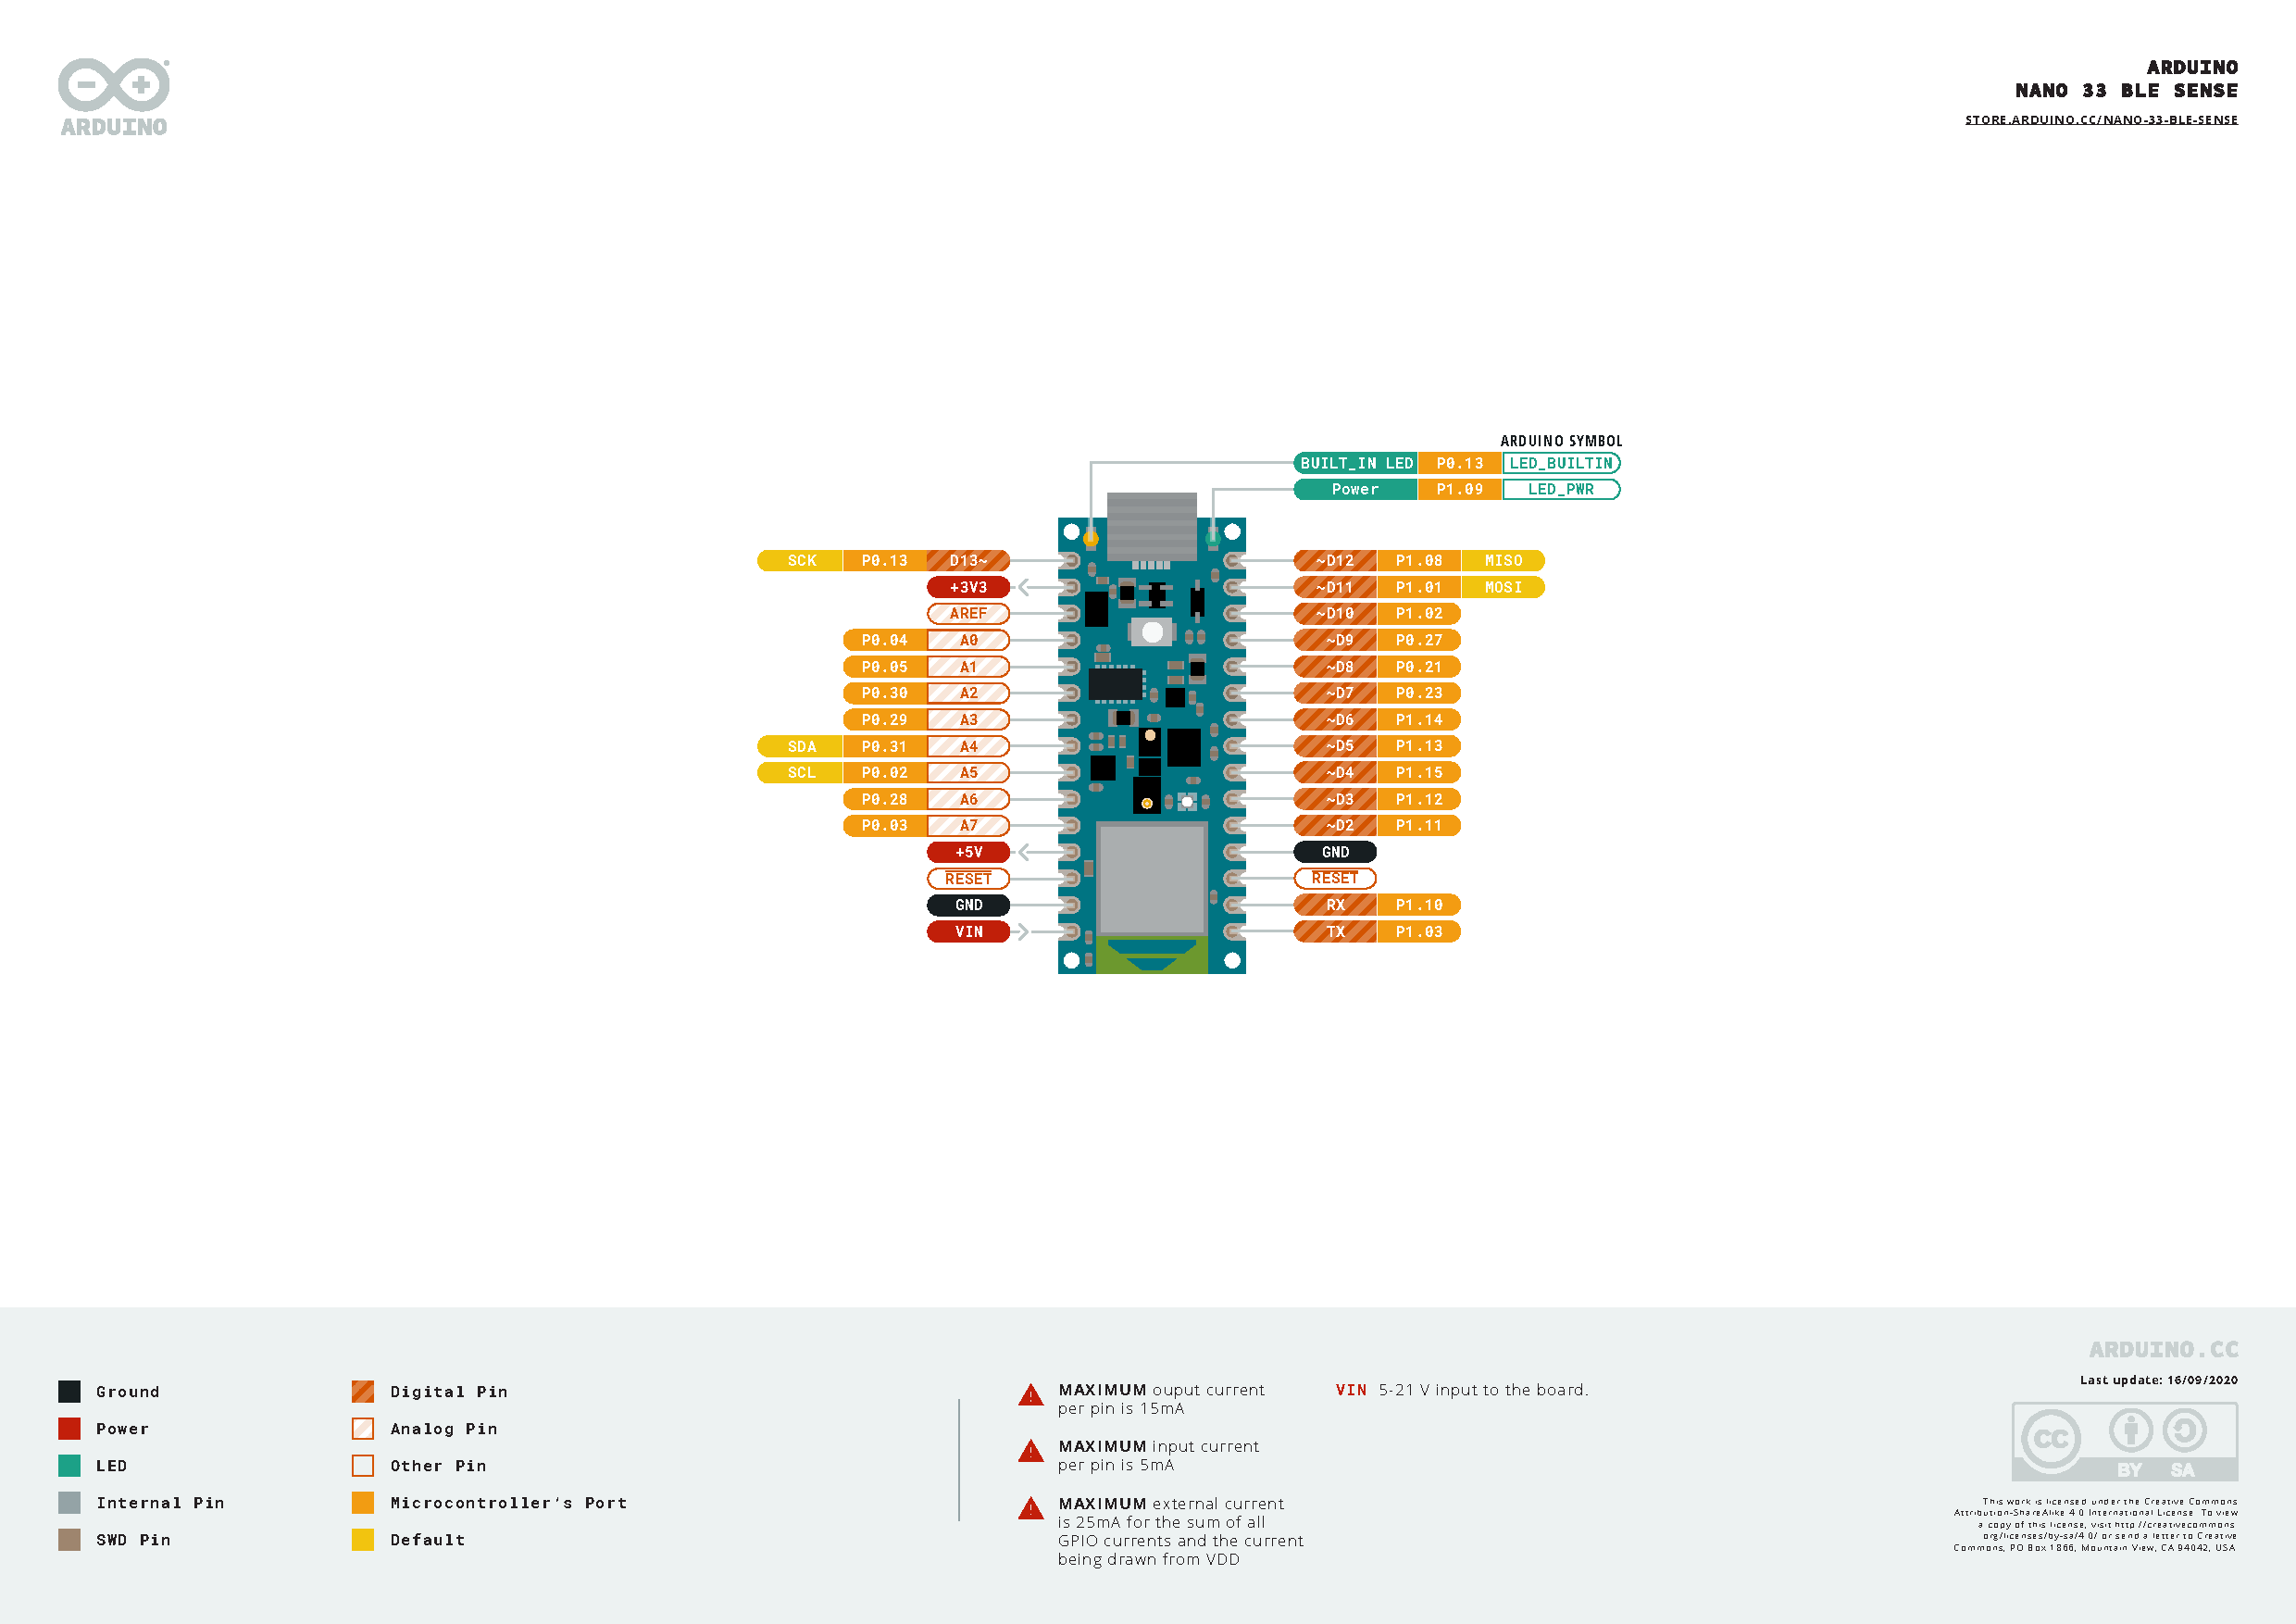
\includepdf[scale=1.0,pages=-,pagecommand=\subsection{Arduino Nano 33 BLE sense PIN layout\label{pinlayout}}]{pdf/Pinout-NANOsense_latest.pdf}


\lstset{frame=tb,
extendedchars = true,
texcl=true,
  language=Bash,
  aboveskip=3mm,
  belowskip=3mm,
  showstringspaces=false,
  columns=flexible,
  basicstyle={\small\ttfamily},
  numbers=none,
  numberstyle=\tiny\color{gray},
  keywordstyle=\color{black},
  commentstyle=\color{dkgreen},
  stringstyle=\color{mauve},
  breaklines=true,
  breakatwhitespace=true,
  tabsize=3
}


\newpage
\section{Maybe useful text}

Thursday 20. August 2020, the group gathered and had a meeting with Steven Bos. We discussed our project idea and the potential use of the Microsoft HoloLens 2. It was in the group's best interest to put our resources into the microcontroller rather than the goggles, dismissing any development with the HoloLens.

\vspace{5mm}
On September 10. the group met to plan the project. After deciding on the initial design, we drew a sketch and wrote a short description. This was sent to our professor, along with a list of required parts as well as the associated budget. The initial design can be seen in section XX.

\vspace{5mm}

On the 16th of September, we ordered three Arduino Nano 33 BLE Sense w/headers from Arduino.cc. This came to 1080NOK. In addition to this the professor provided us with a car for the project. It is called Turnigy Trooper \cite{CAR}, and was originally a radio controlled car. However everything but the battery and servo motors for thrust and steering, have been stripped away. 

The servo motors are controlled by a pulse-width modulated signal. This means in essence that we send discrete signals, where the signal will rise at a fixed frequency. The length of time the signal is high before going low will determine the behaviour of the servo motors. Luckily for us there is a standard regarding the behaviour generated by a specific pulse width. 

We will need to write a library which will abstract this away in the code. Where the interface for steering will take an angle, and the motor interface will hopefully be able to take a velocity in m/s, where negative numbers will mean going backwards.

\vspace{5mm}
%Litt vanskelig med fortid og nåtid i formuleringa her = p
After Steven showed us a proof of concept that it will be quite doable to base our library for the Arduino Nano on the existing toolchain for NRF52840, we started developing on the 17th of September. However there quickly emerged a problem, as Gnat arm-elf initally only supports ZFP-runtime libraries for this card. This meant that it would only support barebone functionality, and we would never be able to make use of the Ada realtime library, or even multithreading the software. Luckily, there exists support for full ravenscar runtime libraries for the card. We followed the official guide at the bb-runtime repo \cite{BBRUNTIMES}, to generate and build them ourselves.

%Before we could start using Ada's real-time library under runtime, we had to generate the library for our microcontroller nRF52840. We followed the official guide [kilde]\url{https://github.com/AdaCore/bb-runtimes} to generate and build the library. 

\begin{lstlisting}
./build_rts.py --rts-src-descriptor ~/opt/GNAT/2020-arm-elf/arm-eabi/lib/gnat/rts-sources.json --output=temp nrf52840
\end{lstlisting}

\begin{lstlisting}
gprbuild -P ~/opt/GNAT/2020-arm-elf/lib/gnat/arm-eabi/lib/gnat/ravenscar-full-nrf52840/ravenscar-build.gpr
\end{lstlisting}


\vspace{5mm}
On the 18th of September we improved our library build, by letting the project\_wizard script in Ada drivers library generate the gpr-files for our board automatically. All we had to do was to provide some basic information about the microcontroller, and the script did the rest. We also started adapting the pin mappings from the nRF52832 to the nRF52840. 

Provided that our efforts lead to a useful library, we will create a pull request into the Ada drivers library, so that others may benefit from our work. 

\begin{lstlisting}
./Ada_Drivers_Library/scripts/project_wizard.py
\end{lstlisting}

\vspace{5mm}

October 5. 

We received the Segger J-Link debugger from our professor. In order to get this to work, we installed the firmware from segger.com. However we also had to install a pack for pyocd in order to find the debugger:


\begin{lstlisting}
pyocd pack --install  stm32l476VG
\end{lstlisting}

As all development within the group is done on Linux, we also had to add udev rules, so that we were able to access the usb ports without being root. These rule-sets were found on pyocds git repository.

We also had to give the respective user access to the serial port by running the command: 
\begin{lstlisting}
usermod -a -G dialout MY\_USER\_NAME
\end{lstlisting}

Legge til utilization test og grafikk.
\vspace{5mm}

October 12. 

We are able to flash and debug by manually holding cables to the debug connections on the Arduino. We used the diagram on the segger website \cite{JLINK} to find out which JLink pins to "connect" to the Arduino points.

AnalogWrite seems like the perfect choice to generate a pulse for both servo and sensor. In the Ada Drivers Library \cite{ADADRIVERSLIBRARY} there is a very good example for controlling a servo. It changes the analog signal period with \textbf{Set\_Analog\_Period\_Us} to generate a steady pulse.

However we were never able to make it work on the arduino. Seems to be a problem with incompatibility between the drivers and the Arduino or the nRF52840 chip.\\
We suspect it is tied to interrupts since the stacktrace from the debugger kept stopping on a new line each time.

Progress is slow because of the manual labour required for each flash and debugging session.
\vspace{5mm}

October 19. 

We recieved the clamps from Richard and Steven was able to put it together with the Arduino and a breadboard. We are finally able to easily flash and debug.

We were able to create a steady pulse using digital I/O and tasks with a fixed priority. With a proper priority we were able to use three tasks for three separate servos and one task for three sensors.

We encountered some problems using a 9V battery power source, as the Ardino requires at least 5V and the peripherals need 5V.


\vspace{5mm}
October 21.

We wrote the code for the entire system.


\vspace{5mm}
October 22.

This was the first day we tested our servo code on the car. After a lot of trial and error on the steering we quickly moved on to the drive motor. We got the wheels to move fairly quickly after discovering that the motor needs a neutral (1500ms PWM) signal to intialize, before giving it signals which indicate torque. However, there quickly emerged problems. First of all the minimum speed was much to high, and secondly, it was impossible to get the car to switch between going forwards and backwards. After conversations with our professor, we learned that Joakim Bjork, had worked a lot with this car, and sat on a lot of documentation for the motors. This documentation would be made available for us on the next day.

\vspace{5mm}

Obtober 23.

\textbf{D-Day} (Documentation day)

\section{Ravenscar}

The full ravenscar runtime library offers what is called the Ravenscar profile. This is a subset of the Ada language, where the features and available libraries are limited. The reason for this is to ensure robust software on realtime and safety critical systems. 

The specifications of the ravenscar profile are the following:
%Lim inn liste kanskje?
https://www.ada-switzerland.ch/rm/RM-D-13.html

There are a couple of limitations here that will affect the way we initially planned our software. 

The maximum number of entries in tasks are set to 0. This means that we won't be able do have dynamic tasking, and all tasks will rather have to be defined at compile-time. 

Another thing we planned was to specify which tasks would run on the respective cores of the CPU. This however, is not supported within the ravenscar profile, and we will need to do all the scheduling as if we only had a single-core processor. 

\subsection{Pin layout}
11.10.2020\\
The nRF52840 has two ports, P0 has 32 pins while P1 has 16 pins.\\ 
We found the P1 base address for the nRF52840 seen on page 23 in the datasheet \cite{NRF52840}. Without it we were only able to use the pins with P0 seen on figure \ref{pinlayout}. After adding the base address to the Ada code and the option to chose between 0 and 47 pin number we were able to make all the pins function.

\end{document}
